\documentclass[11pt, a4paper]{article}

\usepackage{tikz}
\usetikzlibrary{arrows,automata, shapes, petri}

\begin{document}

\title{BACKPROPAGATION}
\date{}
\maketitle

Backpropagation is a computer algorithm used for supervised training of Artificial Neural Networks. It is based on two ideas - the Chain Rule of derivatives in Calculus and Dynamic Programming.

\section{Notation}

\begin{center}
	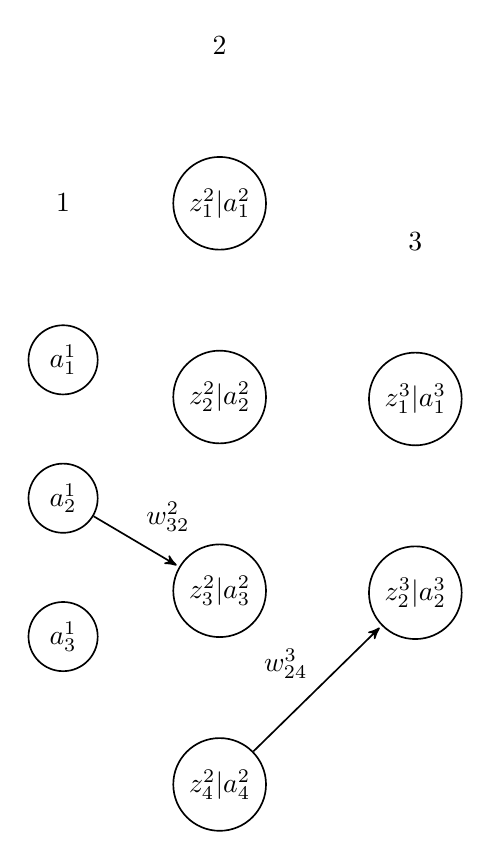
\begin{tikzpicture}[->,>=stealth',shorten >=1pt,auto,
		semithick]
										
		\node[state] (I1)                    {$a^1_1$};
		\node[state] (I2) [below of=I1, node distance=5em] {$a^1_2$};
		\node[state] (I3) [below of=I2, node distance=5em] {$a^1_3$};
		
		\node[state] (J1) [above right of=I1, node distance=8em]  {$z^2_1|a^2_1$};
		\node[state] (J2) [below of=J1, node distance=7em] {$z^2_2|a^2_2$};
		\node[state] (J3) [below of=J2, node distance=7em] {$z^2_3|a^2_3$};
		\node[state] (J4) [below of=J3, node distance=7em] {$z^2_4|a^2_4$};	
		
		\node[state] (K1) [below right of=J1, node distance=10em]  {$z^3_1|a^3_1$};
		\node[state] (K2) [below of=K1, node distance=7em] {$z^3_2|a^3_2$};	
		
		\node [rectangle, node distance=2cm] (I) [above of=I1] {1};
		\node [rectangle, node distance=2cm] (J) [above of=J1] {2};
		\node [rectangle, node distance=2cm] (K) [above of=K1] {3};	
		
		\path (I2) edge  node {$w^2_{32}$} (J3);	
		\path (J4) edge  node {$w^3_{24}$} (K2);		
		                   
	\end{tikzpicture}
\end{center}

The layers are of the Neural Network are denoted by positive integers with input layer denoted by $1$, the first hidden layer by $2$ and so on till the output layer. The inputs in the input layer are denoted by $a^1_{i}$ as shown above. For all the other neurons in other layers, $z^l_i$ denotes the weighted sum of the neuron activations in the previous layer and $a^l_i$ denotes that neuron's activation. The weights are superscripted by the index of the layer of the neuron at the end, and subscripted first by the layer index of the end neuron and then by that of the start neuron.

\section{Forward Propagation}

\end{document}
